\chapter{p3 = 8 (8 graphs)}
\newpage\begin{figure}
  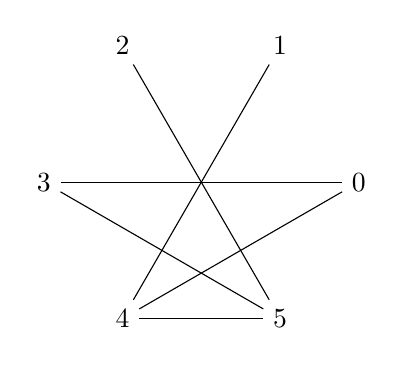
\begin{tikzpicture}
      \draw
        (0.0:2) node (0){0}
        (60.0:2) node (1){1}
        (120.0:2) node (2){2}
        (180.0:2) node (3){3}
        (240.0:2) node (4){4}
        (300.0:2) node (5){5};
      \begin{scope}[-]
        \draw (0) to (3);
        \draw (0) to (4);
        \draw (1) to (4);
        \draw (2) to (5);
        \draw (3) to (5);
        \draw (4) to (5);
      \end{scope}
    \end{tikzpicture}
\end{figure}
\begin{itemize}
\item signature: 001100010001011
\item g: Graph with 6 nodes and 6 edges
\item order: 6
\item size: 6
\item max degree: 3
\item degrees: 1,1,2,2,3,3
\item is tree: 0
\item is bipartite: 1
\item has bridge: 1
\item is chordal: 0
\item is complete: 0
\item min cycle basis weight: 4
\item min cycle basis size: 1
\item diameter: 3
\item radius: 2
\item is eulerian: 0
\item is planar: 1
\item number of faces: 2
\item is regular: 0
\item p3: 8
\item p4: 5
\item property hash: b060646e78d8dc5a1c3eb0da2631b41db48c8a8a602bb16755891f3e6b4cfb7d
\end{itemize}
\newpage
\begin{figure}
  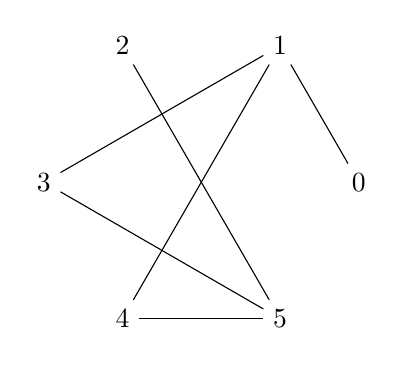
\begin{tikzpicture}
      \draw
        (0.0:2) node (0){0}
        (60.0:2) node (1){1}
        (120.0:2) node (2){2}
        (180.0:2) node (3){3}
        (240.0:2) node (4){4}
        (300.0:2) node (5){5};
      \begin{scope}[-]
        \draw (0) to (1);
        \draw (1) to (3);
        \draw (1) to (4);
        \draw (2) to (5);
        \draw (3) to (5);
        \draw (4) to (5);
      \end{scope}
    \end{tikzpicture}
\end{figure}
\begin{itemize}
\item signature: 100000110001011
\item g: Graph with 6 nodes and 6 edges
\item order: 6
\item size: 6
\item max degree: 3
\item degrees: 1,1,2,2,3,3
\item is tree: 0
\item is bipartite: 1
\item has bridge: 1
\item is chordal: 0
\item is complete: 0
\item min cycle basis weight: 4
\item min cycle basis size: 1
\item diameter: 4
\item radius: 2
\item is eulerian: 0
\item is planar: 1
\item number of faces: 2
\item is regular: 0
\item p3: 8
\item p4: 4
\item property hash: b0278d13cadf5f98ed8fe1e3943a9114e5bf491ae05d4956905101c17585c3d1
\end{itemize}
\newpage
\begin{figure}
  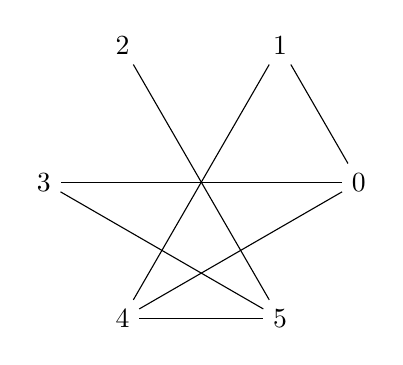
\begin{tikzpicture}
      \draw
        (0.0:2) node (0){0}
        (60.0:2) node (1){1}
        (120.0:2) node (2){2}
        (180.0:2) node (3){3}
        (240.0:2) node (4){4}
        (300.0:2) node (5){5};
      \begin{scope}[-]
        \draw (0) to (1);
        \draw (0) to (3);
        \draw (0) to (4);
        \draw (1) to (4);
        \draw (2) to (5);
        \draw (3) to (5);
        \draw (4) to (5);
      \end{scope}
    \end{tikzpicture}
\end{figure}
\begin{itemize}
\item signature: 101100010001011
\item g: Graph with 6 nodes and 7 edges
\item order: 6
\item size: 7
\item max degree: 3
\item degrees: 1,2,2,3,3,3
\item is tree: 0
\item is bipartite: 0
\item has bridge: 1
\item is chordal: 0
\item is complete: 0
\item min cycle basis weight: 7
\item min cycle basis size: 2
\item diameter: 3
\item radius: 2
\item is eulerian: 0
\item is planar: 1
\item number of faces: 3
\item is regular: 0
\item p3: 8
\item p4: 5
\item property hash: bf9d325043ba78e41e44f32e29357a2269ef2b904a42a0e6eeb33494b04b7dcc
\end{itemize}
\newpage
\begin{figure}
  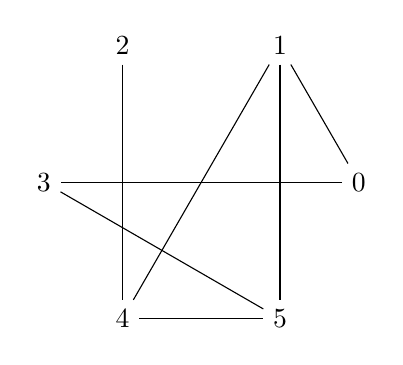
\begin{tikzpicture}
      \draw
        (0.0:2) node (0){0}
        (60.0:2) node (1){1}
        (120.0:2) node (2){2}
        (180.0:2) node (3){3}
        (240.0:2) node (4){4}
        (300.0:2) node (5){5};
      \begin{scope}[-]
        \draw (0) to (1);
        \draw (0) to (3);
        \draw (1) to (4);
        \draw (1) to (5);
        \draw (2) to (4);
        \draw (3) to (5);
        \draw (4) to (5);
      \end{scope}
    \end{tikzpicture}
\end{figure}
\begin{itemize}
\item signature: 101000011010011
\item g: Graph with 6 nodes and 7 edges
\item order: 6
\item size: 7
\item max degree: 3
\item degrees: 1,2,2,3,3,3
\item is tree: 0
\item is bipartite: 0
\item has bridge: 1
\item is chordal: 0
\item is complete: 0
\item min cycle basis weight: 7
\item min cycle basis size: 2
\item diameter: 3
\item radius: 2
\item is eulerian: 0
\item is planar: 1
\item number of faces: 3
\item is regular: 0
\item p3: 8
\item p4: None
\item property hash: 4f38d06952c37c157ff19cd97f9e2b85cec6c44791aa5c00bd60fd3804e7487b
\end{itemize}
\newpage
\begin{figure}
  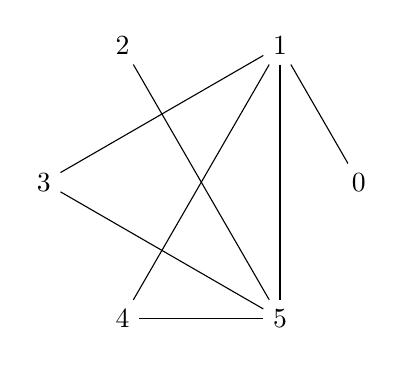
\begin{tikzpicture}
      \draw
        (0.0:2) node (0){0}
        (60.0:2) node (1){1}
        (120.0:2) node (2){2}
        (180.0:2) node (3){3}
        (240.0:2) node (4){4}
        (300.0:2) node (5){5};
      \begin{scope}[-]
        \draw (0) to (1);
        \draw (1) to (3);
        \draw (1) to (4);
        \draw (1) to (5);
        \draw (2) to (5);
        \draw (3) to (5);
        \draw (4) to (5);
      \end{scope}
    \end{tikzpicture}
\end{figure}
\begin{itemize}
\item signature: 100000111001011
\item g: Graph with 6 nodes and 7 edges
\item order: 6
\item size: 7
\item max degree: 4
\item degrees: 1,1,2,2,4,4
\item is tree: 0
\item is bipartite: 0
\item has bridge: 1
\item is chordal: 1
\item is complete: 0
\item min cycle basis weight: 6
\item min cycle basis size: 2
\item diameter: 3
\item radius: 2
\item is eulerian: 0
\item is planar: 1
\item number of faces: 3
\item is regular: 0
\item p3: 8
\item p4: None
\item property hash: deb555b546c98a4d7fe5c31e0ef7355e882f0c17a6a064457ac1b0d7e4f8c484
\end{itemize}
\newpage
\begin{figure}
  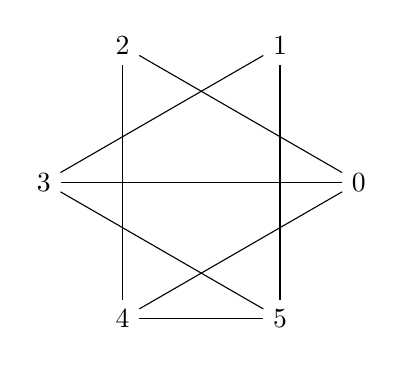
\begin{tikzpicture}
      \draw
        (0.0:2) node (0){0}
        (60.0:2) node (1){1}
        (120.0:2) node (2){2}
        (180.0:2) node (3){3}
        (240.0:2) node (4){4}
        (300.0:2) node (5){5};
      \begin{scope}[-]
        \draw (0) to (2);
        \draw (0) to (3);
        \draw (0) to (4);
        \draw (1) to (3);
        \draw (1) to (5);
        \draw (2) to (4);
        \draw (3) to (5);
        \draw (4) to (5);
      \end{scope}
    \end{tikzpicture}
\end{figure}
\begin{itemize}
\item signature: 011100101010011
\item g: Graph with 6 nodes and 8 edges
\item order: 6
\item size: 8
\item max degree: 3
\item degrees: 2,2,3,3,3,3
\item is tree: 0
\item is bipartite: 0
\item has bridge: 0
\item is chordal: 0
\item is complete: 0
\item min cycle basis weight: 10
\item min cycle basis size: 3
\item diameter: 3
\item radius: 2
\item is eulerian: 0
\item is planar: 1
\item number of faces: 4
\item is regular: 0
\item p3: 8
\item p4: 6
\item property hash: f3a6df97b34c34621f3f21cfa59b00ecf9d13fe7b47135f9aa1d731b58779ead
\end{itemize}
\newpage
\begin{figure}
  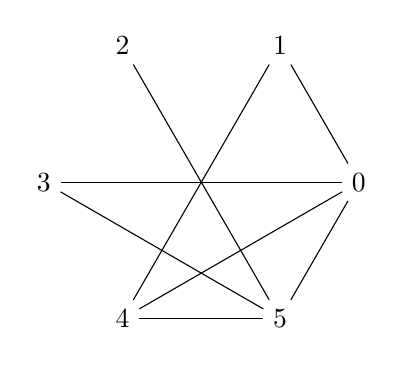
\begin{tikzpicture}
      \draw
        (0.0:2) node (0){0}
        (60.0:2) node (1){1}
        (120.0:2) node (2){2}
        (180.0:2) node (3){3}
        (240.0:2) node (4){4}
        (300.0:2) node (5){5};
      \begin{scope}[-]
        \draw (0) to (1);
        \draw (0) to (3);
        \draw (0) to (4);
        \draw (0) to (5);
        \draw (1) to (4);
        \draw (2) to (5);
        \draw (3) to (5);
        \draw (4) to (5);
      \end{scope}
    \end{tikzpicture}
\end{figure}
\begin{itemize}
\item signature: 101110010001011
\item g: Graph with 6 nodes and 8 edges
\item order: 6
\item size: 8
\item max degree: 4
\item degrees: 1,2,2,3,4,4
\item is tree: 0
\item is bipartite: 0
\item has bridge: 1
\item is chordal: 1
\item is complete: 0
\item min cycle basis weight: 9
\item min cycle basis size: 3
\item diameter: 3
\item radius: 2
\item is eulerian: 0
\item is planar: 1
\item number of faces: 4
\item is regular: 0
\item p3: 8
\item p4: None
\item property hash: 2dc5289ca64bdd886b925f1006ebd6c9713a25464c21edc8432fcf6414f528b4
\end{itemize}
\newpage
\begin{figure}
  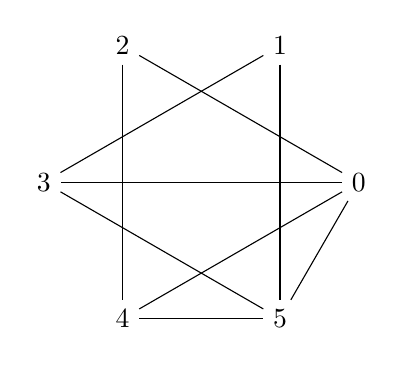
\begin{tikzpicture}
      \draw
        (0.0:2) node (0){0}
        (60.0:2) node (1){1}
        (120.0:2) node (2){2}
        (180.0:2) node (3){3}
        (240.0:2) node (4){4}
        (300.0:2) node (5){5};
      \begin{scope}[-]
        \draw (0) to (2);
        \draw (0) to (3);
        \draw (0) to (4);
        \draw (0) to (5);
        \draw (1) to (3);
        \draw (1) to (5);
        \draw (2) to (4);
        \draw (3) to (5);
        \draw (4) to (5);
      \end{scope}
    \end{tikzpicture}
\end{figure}
\begin{itemize}
\item signature: 011110101010011
\item g: Graph with 6 nodes and 9 edges
\item order: 6
\item size: 9
\item max degree: 4
\item degrees: 2,2,3,3,4,4
\item is tree: 0
\item is bipartite: 0
\item has bridge: 0
\item is chordal: 1
\item is complete: 0
\item min cycle basis weight: 12
\item min cycle basis size: 4
\item diameter: 3
\item radius: 2
\item is eulerian: 0
\item is planar: 1
\item number of faces: 5
\item is regular: 0
\item p3: 8
\item p4: 5
\item property hash: ee13cfbf2908fe8a1e5bcf79c637bb8c3b3f0e9bb783751d5dd737357a5faab4
\end{itemize}
\newpage
